\section{Image processing and information extraction}\label{sec:improc}

\subsection{Simple calculus with channels}\label{ssec:calculus}

The \application{BandMath} application provides a simple and efficient
way to perform band operations. The command line application and the
corresponding Monteverdi module (shown in the section \ref{Band_math module})
are based on the same standards. It computes a band wise operation according
to a user defined mathematical expression. The following code computes the
absolute difference between first bands of two images:

\begin{verbatim}
otbcli_BandMath -il input_image_1 input_image_2
                -exp "abs(im1b1 - im2b1)"
                -out output_image
\end{verbatim}

The naming convention "im[x]b[y]" designates the yth band of the xth input image.

The \application{BandMath} application embeds built-in operators and functions
(listed \href{http://muparser.sourceforge.net/mup_features.html#idDef2}{here}),
allowing a vast choice of possible operations.

\subsection{Segmentation}\label{ssec:segmentation}

Segmenting objects across a very high resolution scene and with a controlled
quality is a difficult task for which no method has reached a sufficient level
of performance to be considered as operational.

Even if we leave aside the question of segmentation quality and
consider that we have a method performing reasonably well on our data
and objects of interest, the task of scaling up segmentation to real
very high resolution data is itself challenging. First, we can not
load the whole data into memory, and there is a need for on the flow
processing which does not cope well with traditional segmentation
algorithms. Second, the result of the segmentation process
itself is difficult to represent and manipulate efficiently.

The experience of segmenting large remote sensing images is packed into a single
\application{Segmentation} in \app.

You can find more information about this application
\href{http://blog.orfeo-toolbox.org/preview/coming-next-large-scale-segmentation}{here}.

\subsection{Classification}\label{ssec:classification}

The SVM classification in application framework provides a supervised pixel-wise
classification chain based on learning from multiple images. It supports huge
images through streaming and multi-threading.
The classification chain performs a SVM training step based on the intensities
of each pixel as features. Please note that all the input images must have the
same number of bands to be comparable.

\subsubsection{Statistics estimation}
In order to make these features comparable between each images, the first step
is to estimate the input images statistics. These statistics will be used to
center and reduce the intensities (mean of 0 and standard deviation of 1) of
samples based on the vector data produced by the user. To do so, the
\application{ComputeImagesStatistics} tool can be used :

\begin{verbatim}
otbcli_ComputeImagesStatistics -il  list_of_input_images
                               -out statistics.xml
\end{verbatim}

This tool will compute each band mean, compute the standard deviation based on
pooled variance of each band and finally export them to an XML file.
The features statistics XML file will be an input of the following tools.

\subsubsection{Building the training data set}

As the chain is supervised, we need first to build a training set with
positive examples of different objects of interest. This can be done
with Monteverdi Vectorization module
(Fig.\ref{fig:vectoModuleDataSetCreation}).
These polygons must be save in OGR vector format supported
by GDAL like ESRI shapefile for example.

This operation will be reproduced on each image used as input of the training
function.

Please note that the positive examples in the vector data should have a ``Class``
field with a label value higher than 1 and coherent in each images.

\begin{figure}
  \center
  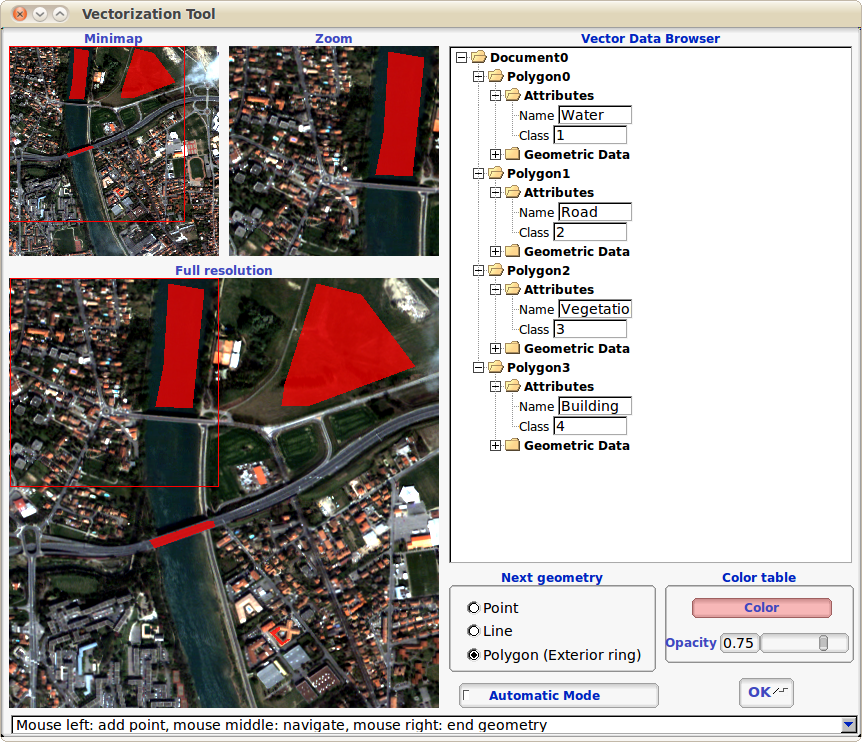
\includegraphics[width=1\textwidth]{../Art/MonteverdiImages/monteverdi_vectorization_module_for_classification.png}
  \itkcaption[GUI of the vectorization module with data for classification chain]{A training data set builded with the vectorization monteverdi module.}
  \label{fig:vectoModuleDataSetCreation}
\end{figure}

You can generate the vector data set with \qgis software for
example and save it in an OGR vector format supported by \gdal (ESRI
sphapefile for example). \app should be able to transform the
vector data into the image coordinate system.

\subsubsection{Performing the learning scheme}

Once images statistics have been estimated, the learning scheme is the following:
\begin{enumerate}
  \item For each input image:
  \begin{enumerate}
    \item Read the region of interest (ROI) inside the shapefile,
    \item Generate validation and training data within the ROI,
    \item Add vectors respectively to the training samples set and the validation
    samples set.
  \end{enumerate}
  \item Increase the size of the training samples set and balance it by
  generating new noisy samples from the previous ones,
  \item Perform the learning with this training set
  \item Estimate performances of the classifier on the validation samples set
  (confusion matrix, precision, recall and F-Score).
\end{enumerate}

These steps can be performed by the \application{TrainSVMImagesClassifier}
command-line using the following:

\begin{verbatim}
otbcli_TrainSVMImagesClassifier -io.imstat  images_statistics.xml
                                -io.il  list_of_input_images
                                -io.vd  list_of_positive_examples_shapefiles
                                -io.out model.svm
\end{verbatim}

Optionnal groups of parameters are also available (see application help for
more details):
\begin{itemize}
\item \verb?-elev? Handling of elevation (DEM or average elevation)
\item \verb?-sample? Group of parameters for sampling
\item \verb?-svm? Group of parameters for SVM
\end{itemize}

\subsubsection{Validating the classification model}
It is also possible to estimate the performance of the SVM model with a
new validation sample set and another image with the
\application{ValidateSVMImagesClassifier} application. It will compute
the global confusion matrix and precision, recall and F-score of each
class based on the \href{http://www.orfeo-toolbox.org/doxygen-current/classotb_1_1ConfusionMatrixCalculator.html}{ConfusionMatrixCalculator}
class.

\begin{verbatim}
otbcli_ValidateSVMImagesClassifier -imstat  images_statistics.xml
                                   -svm model.svm
                                   -il  input_image_list
                                   -vd  list_of_positive_examples_shapefiles
\end{verbatim}

You can save these results with the option -out output filename.
%You can also set a DEM repository (-dem) to keep the vectordata reprojection accurate.

\subsubsection{Using the classification model}
Once the classifier has been trained, one can apply the model to classify
pixel inside defined classes on a new image using the
\application{ImageSVMClassifier} application:

\begin{verbatim}
otbcli_ImageSVMClassifier -imstat  images_statistics.xml
                          -svm model.svm
                          -in  input_image
                          -out labeled_image
\end{verbatim}

You can set an input mask to limit the classification to the mask area with
value \textgreater 0.

\subsubsection{Fancy classification results}

Color mapping can be used to apply color transformations on the final
graylevel label image. It allows to get an RGB classification map
by re-mapping the image values to be suitable for display purposes.
One can use the \application{ColorMapping} application. This tool will
replace each label with an 8-bits RGB color specificied in a mapping
file. The mapping file should look like this :

\begin{verbatim}
# Lines beginning with a # are ignored
1 255 0 0
\end{verbatim}

In the previous example, 1 is the label and 255 0 0 is a RGB color
(this one will be rendered as red). To use the mapping tool, enter
the following :

\begin{verbatim}
otbcli_ColorMapping -in  labeled_image
                    -out color_image
                    -method custom
                    -method.custom.lut  mapping_file
\end{verbatim}

Other look-up tables (LUT) are available : standard continuous LUT,
optimal LUT, and LUT computed over a support image.

\subsubsection{Example}
We take 4 classes: water, roads, vegetation and buildings with red roof.
Data is available in the OTB-Data
\href{http://hg.orfeo-toolbox.org/OTB-Data/file/0fed8f4f035c/Input/Classification}{repository}
and this image is produced with the commands inside this
\href{http://hg.orfeo-toolbox.org/OTB-Applications/file/3ce975605013/Testing/Classification/CMakeLists.txt}{file}.

\begin{figure}[!h]
  \center
  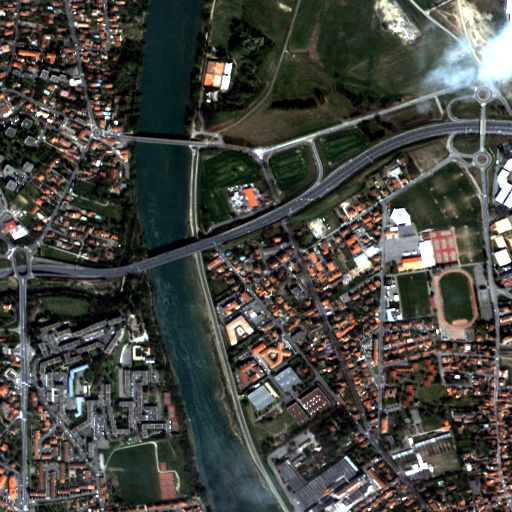
\includegraphics[width=0.3\textwidth]{../Art/MonteverdiImages/classification_chain_inputimage.jpg}
  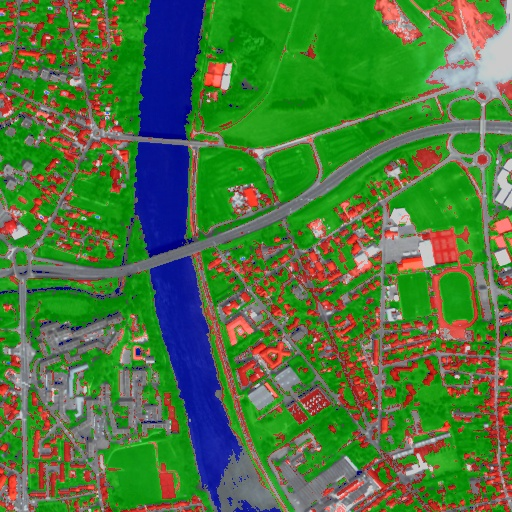
\includegraphics[width=0.3\textwidth]{../Art/MonteverdiImages/classification_chain_fancyclassif_fusion.jpg}
  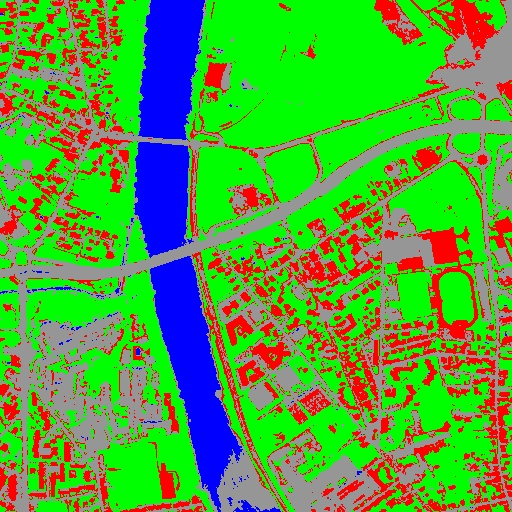
\includegraphics[width=0.3\textwidth]{../Art/MonteverdiImages/classification_chain_fancyclassif.jpg}
  \itkcaption[ExampleSVMCalssif]{From left to right: Original image,
    result image with fusion (with monteverdi viewer) of original
    image and fancy classification and input image with fancy color
    classification from labeled image.}
  \label{fig:MeanShiftVectorImageFilter}
\end{figure}



%\subsection{Segmentation}\label{ssec:segmentation}
%todo.

%\subsection{Change detection}\label{ssec:changedetection}
%todo.

%\subsection{Object-based image analysis}\label{ssec:obia}
%todo.

\subsection{Dempster Shafer based Classifier Fusion}\label{ssec:classifierfusion}

This framework is dedicated to perform cartographic validation starting
from the result of a detection (for example a road extraction), enhance
the results fiability by using a classifier fusion algorithm. Using a
set of descriptor, the processing chain validates or invalidates the
input geometrical features.

% \subsubsection{Prequel: Road Extraction}
%
% The first step of this recipe is to produce an interesting and adapted
% input. The \application{otbRoadExtractionApplication},  included in
% \app , provides a set of geometrical features that can be used as input of the following process. This is only an example, the Dempster-Shafer framework was not designed specifically to be used with otbRoadExtractionApplication but it is a good example of what the input should be like.

\subsubsection{Fuzzy Model (requisite)}

The \application{DSFuzzyModelEstimation} application performs the fuzzy
model estimation (once by use case: descriptor set / Belief support /
Plausibility support). It has the following input parameters :
\begin{itemize}
\item \verb?-psin? a vector data of positive samples enriched according to the
"Compute Descriptors" part
\item \verb?-nsin? a vector data of negative samples enriched according to the
"Compute Descriptors" part
\item \verb?-belsup? a support for the Belief computation
\item \verb?-plasup? a support for the Plausibility computation
\item \verb?-desclist? an initialization model (xml file) or a descriptor name list
(listing the descriptors to be included in the model)
\end{itemize}

The application can be used like this:
\begin{verbatim}
otbcli_DSFuzzyModelEstimation -psin     PosSamples.shp
                              -nsin     NegSamples.shp
                              -belsup   "ROADSA"
                              -plasup   "NONDVI" "ROADSA" "NOBUIL"
                              -desclist "NONDVI" "ROADSA" "NOBUIL"
                              -out      FuzzyModel.xml
\end{verbatim}

The output file \verb?FuzzyModel.xml? contains the optimal model to perform
informations fusion.

\subsubsection{First Step: Compute Descriptors}

The first step in the classifier fusion based validation is to compute, for
each studied polyline, the choosen descriptors. In this context, the
\application{ComputePolylineFeatureFromImage} application can be used for a
large range of descriptors. It has the following inputs :
\begin{itemize}
\item \verb?-in? an image (of the sudied scene) corresponding to the choosen
descriptor (NDVI, building Mask\dots)
\item \verb?-vd? a vector data containing polyline of interest
\item \verb?-expr? a formula ("b1 \textgreater 0.4", "b1 == 0") where b1 is
the standard name of input image first band
\item \verb?-field? a field name corresponding to the descriptor codename
(NONDVI, ROADSA...)
\end{itemize}

The output is a vector data containing polylines with a new field containing
the descriptor value. In order to add the "NONDVI" descriptor to an input
vector data ("inVD.shp") corresponding to the percentage of pixels along a
polyline that verifies the formula "NDVI \textgreater 0.4" :

\begin{verbatim}
otbcli_ComputePolylineFeatureFromImage -in   NDVI.TIF
                                       -vd  inVD.shp
                                       -expr  "b1 > 0.4"
                                       -field "NONDVI"
                                       -out   VD_NONDVI.shp
\end{verbatim}

\verb?NDVI.TIF? is the NDVI mono band image of the studied scene.
This step must be repeated for each choosen descriptor:

\begin{verbatim}
otbcli_ComputePolylineFeatureFromImage -in   roadSpectralAngle.TIF
                                       -vd  VD_NONDVI.shp
                                       -expr  "b1 > 0.24"
                                       -field "ROADSA"
                                       -out   VD_NONDVI_ROADSA.shp
\end{verbatim}

\begin{verbatim}
otbcli_ComputePolylineFeatureFromImage -in   Buildings.TIF
                                       -vd  VD_NONDVI_ROADSA.shp
                                       -expr  "b1 == 0"
                                       -field "NOBUILDING"
                                       -out   VD_NONDVI_ROADSA_NOBUIL.shp
\end{verbatim}

Both \verb?NDVI.TIF? and \verb?roadSpectralAngle.TIF? can be produced
using \mont feature extraction capabilities, and \verb?Buildings.TIF?
can be generated using \mont rasterization module. From now on,
\verb?VD_NONDVI_ROADSA_NOBUIL.shp? contains three descriptor fields.
It will be used in the following part.

\subsubsection{Second Step: Feature Validation}

The final application (\application{VectorDataDSValidation}) will
validate or unvalidate the studied samples using
\href{http://en.wikipedia.org/wiki/Dempster\%E2\%80\%93Shafer_theory}{the Dempster-Shafer theory}
. Its inputs are :
\begin{itemize}
\item \verb?-in? an enriched vector data "VD\_NONDVI\_ROADSA\_NOBUIL.shp"
\item \verb?-belsup? a support for the Belief computation
\item \verb?-plasup? a support for the Plausibility computation
\item \verb?-descmod? a fuzzy model FuzzyModel.xml
\end{itemize}
The output is a vector data containing only the validated samples.

\begin{verbatim}
otbcli_VectorDataDSValidation -in      extractedRoads_enriched.shp
                              -descmod FuzzyModel.xml
                              -out     validatedSamples.shp
\end{verbatim}

\subsection{Stereo reconstruction from VHR optical image pair}\label{sec:stereoreconstruction}

This section describes how to convert pair of images into elevation information.

\subsubsection{First step: estimate epipolar geometry transformation}\label{ssec:epipolar}
The aim of this application is to generate resampling grids to transform images
in epipolar geometry.  Epipolar geometry is the geometry of stereo vision (see
\href{http://en.wikipedia.org/wiki/Epipolar_geometry}). The operation of stereo
rectification determines a transformation of each image plane such that pairs of
conjugate epipolar lines become collinear and parallel to one of the image axes.

After applying this transformation, it reduces the problem of elevation (or
stereo correspondences determination) to a 1-D problem.  We've got two images
image1 and image2 over the same area (the stereo pair) and we assume that we
know the localization functions (forward and inverse) associated for each of
these images.

The forward function allows to go from the image referential to the geographic
referential:
\begin{equation}
  (long,lat) = f^{forward}_{image1}(i,j,h)
\end{equation}

where h is the elevation hypothesis, (i, j) are the pixel coordinates in image1
and (long,lat) are geographic coordinates.  As you can imagine, the inverse
function allows to go from geographic coordinates to the image geometry.

For the second image:

\begin{equation}
   (long,lat,h) = f^{inverse}_{image2}(i,j)
\end{equation}

Using jointly the forward and inverse functions from the image pair, we can
construct a co-localization function $f_{image1 \rightarrow image2}$ between a
the position of a pixel in the first and its position in the second one:

\begin{equation}
(i_{image2},j_{image2}) = f_{image1 \rightarrow image2} (i_{image1} , j_{image1} , h)
\end{equation}

The expression of this function is:

\begin{equation}
f_{image1 \rightarrow image2} (i_{image1} , j_{image1} , h) =  f^{inverse}_{image2} f^{forward}_{image1}((i_{image1} , j_{image1}), h)
\end{equation}

The expression is not really important, what we need to understand is that if we
are now able to determine for a given pixel in image1 the corresponding pixel in
image2.  As we know the expression of co-localization function between images,
we've got the information about the elevation (variable h in the equation)!

We've got now the mathematical basis to understand how 3-D information can be
extracted by examination of the relative positions of objects in the two 2-D
images.

The construction of the two epipolar grids is a little bit more complicated in
case of VHR optical images.That's because most of passive remote sensing from
space use a push broom sensor, which corresponds to a line of sensors arranged
perpendicular to the flight direction of the spacecraft. This acquisition
configuration implies a slightly different strategy for stereo-rectification
(see details here :
\href{http://en.wikipedia.org/wiki/Epipolar_geometry#Epipolar_geometry_of_pushbroom_sensor}).

Let's examine now how to use the \application{StereoRectificationGridGenerator}
application to produce two images which are \textgreater{deformation grids} for
image1 and image2.

\begin{verbatim}
otbcli_StereoRectificationGridGenerator -io.inleft image1.tif
                                        -io.inright image1.tif
                                        -epi.elevation.avg.value 100
                                        -epi.step 10
                                        -io.outimage1 outimage1_grid.tif
                                        -io.outright outimage1_grid.tif
\end{verbatim}

The application estimates a displacement to apply for each pixel in the two
input images to obtain epipolar geometry.You can see that the application can
accept a `step' parameter to estimate displacements on a coarser grid. Here we
estimate the displacements every 10 pixel. That's because in most cases with a
pair of VHR and a small angle between the two images, this grid is almost
regular.  Moreover, the implementation is not \textit{streamable} and use potentially a
lot of memory. So that, it is generally a good idea to estimate the displacement
grid at a coarser resolution.

The application outputs the size of the output image in epipolar
geometry. \textbf{Note these values}, we will use it at the next step to
resample the two images in epipolar geometry.

In my case, I've got:

\begin{verbatim}
Output parameters value:
epi.rectsizex: 4464
epi.rectsizey: 2958
epi.baseline: 4.772260666
\end{verbatim}

Moreover the epi.baseline parameter provides the mean value, in meters, of the
baseline to sensor altitude ratio. It can be used to convert disparities to
physical elevation, since a disparity of one pixel will correspond to an
elevation offset of this value with respect to the mean elevation.

Let's move forward to the resampling in epipolar geometry.

\subsubsection{Resample images in epipolar geometry}

The prior application generates two grids of displacements. The
\application{GridBasedImageResampling} allows to resample the two input images
in the epipolar geometry using these grids.  These grids are intermediary result
not really useful as it in most cases. This second step \textit{only} consists in
applying the transformation and resample both images but this application can be
useful in a lot of other cases.

The two commands to generate epipolar images are:
\begin{verbatim}
otbcli_GridBasedImageResampling -io.in image1.tif
                                -io.out image1_epipolar.tif
                                -grid.in outimage1_grid.tif
                                -out.sizex 4464
                                -out.sizey 2958
\end{verbatim}

\begin{verbatim}
otbcli_GridBasedImageResampling -io.in image2.tif
                                -io.out image2_epipolar.tif
                                -grid.in outimage2_grid.tif
                                -out.sizex 4464
                                -out.sizey 2958
\end{verbatim}

As you can see, we set sizex and sizey parameters using output values given by
the \application{StereoRectificationGridGenerator} application to set the size
of the output epipolar images.

\begin{figure}[!h]
  \center
  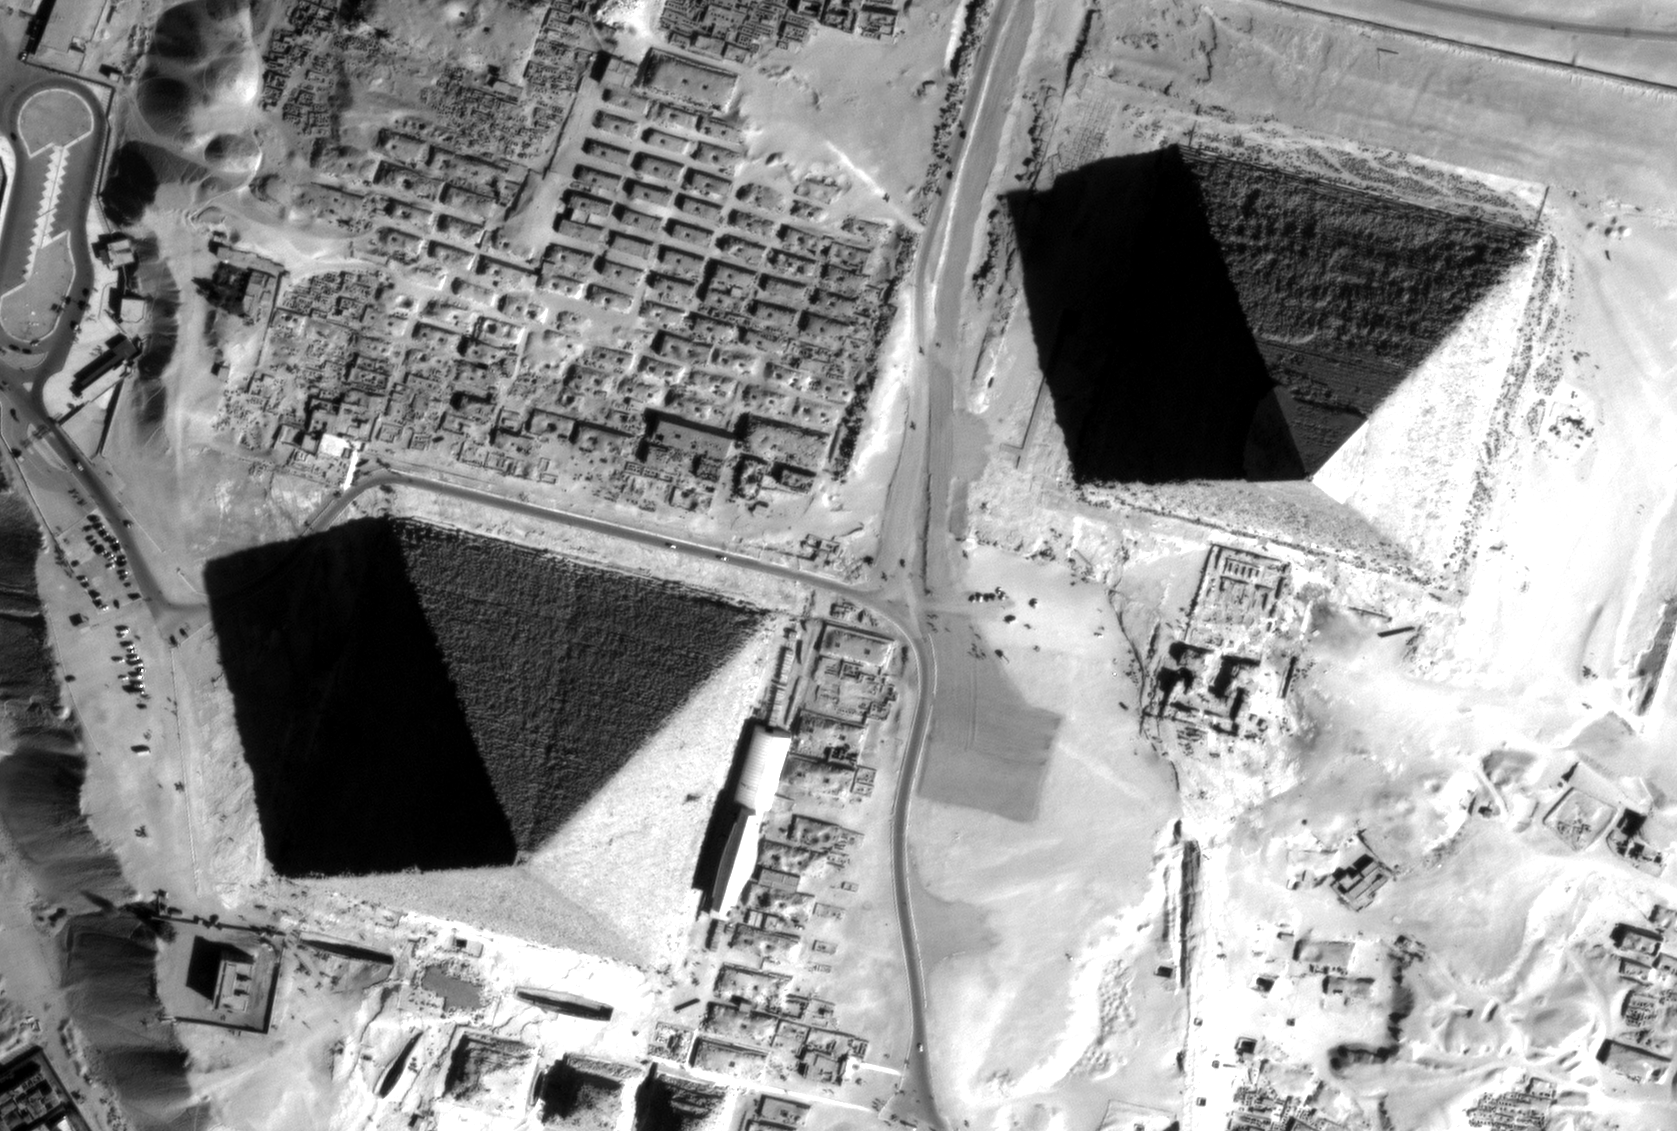
\includegraphics[width=0.45\textwidth]{../Art/MonteverdiImages/stereo_image1_epipolar.png}
  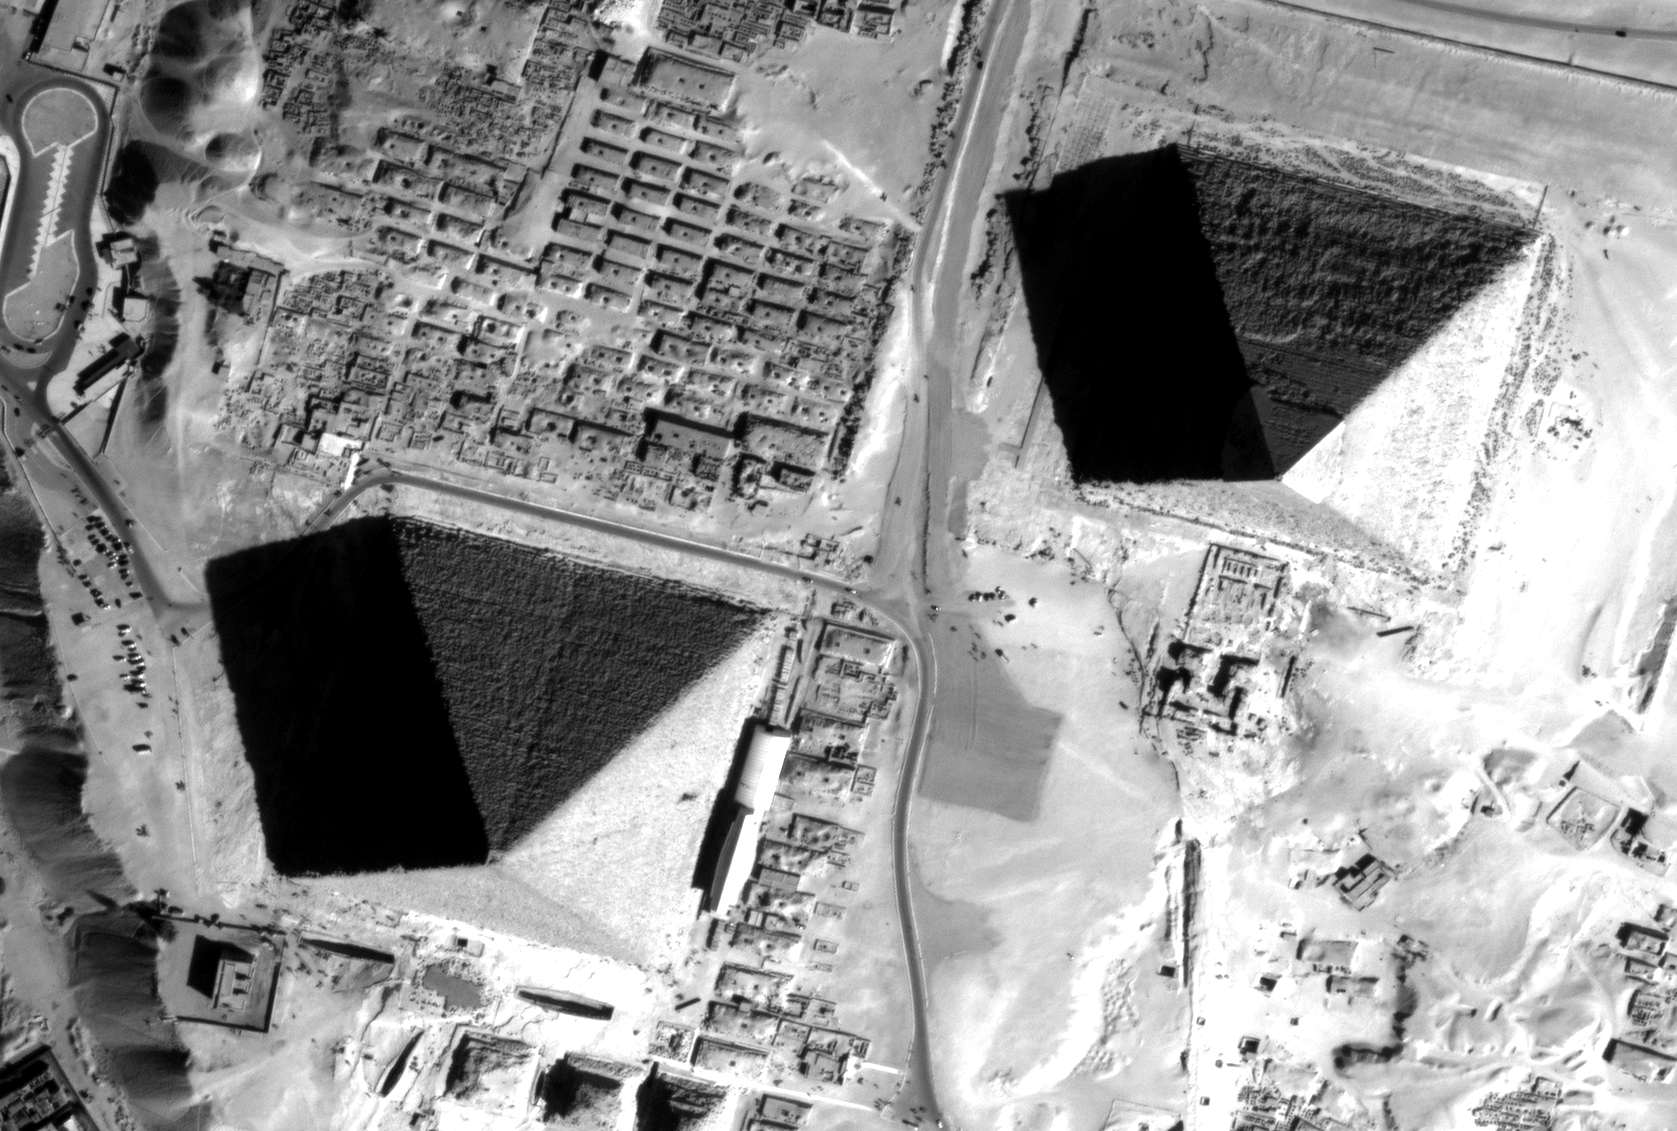
\includegraphics[width=0.45\textwidth]{../Art/MonteverdiImages/stereo_image2_epipolar.png}
  \itkcaption[ExampleEpipolar]{Extract of resample image1 and image2 in epipolar geometry over Pyramids of
Cheops.}
  \label{fig:MeanShiftVectorImageFilter}
\end{figure}

\subsubsection{Disparity estimation: Block matching on epipolar lines}

Finally, we can begin the stereo correspondences! Things become a little are
more complicated but lets describe now the powerfulness of the
\application{BlockMatching} application.  To correlate block from the first
image with a block in the second image, we've got two epipolar data where the
use of epipolar lines allows us to constrain the search along a 1-dimensional
line as opposed to the entire 2-dimensional image. Moreover, block matching is
used, as opposed to single point matching, because of the obvious advantage that
correlating blocks is much more likely to reflect a true match.

For each point in the first image (the \textit{baseline}), we can search for the
corresponding pixel in the second image and use the co-localization function
describes in \ref{ssec:epipolar}.

An almost complete spectrum of stereo correspondence algorithms has been
published and it is still augmented at a significant rate!See for example
\href{http://en.wikipedia.org/wiki/Block-matching_algorithm} for example. The
\otb implements different strategies for block matching:

\begin{itemize}
\item Sum of Square Distances block-matching (SSD)
\item Normalized Cross-Correlation (NCC)
\item Lp pseudo-norm (LP)
\end{itemize}

An other important mandatory parameter of the application is the range of
disparities. In theory, the block matching can perform a blind exploration and
search for a infinite range of disparities between the stereo pair. We need now
to evaluate the range of disparities where the block (from the deepest point on
Earth, the Challenger Deep (\url{http://en.wikipedia.org/wiki/Challenger_Deep})
to the Everest summit!  I deliberately exaggerated but you can imagine that with
a smaller range you can imagine that the block matching algorithm can take a lot
of time.  That's why these parameters are mandatory for the application and as
consequence we need to estimate them manually. That's pretty simple using the
two epipolar images.

In my case, I take one point on a flat area. The image coordinate in $image_{1}$
is $[1970,1525]$ and in $image_{2}$ is $[1970,1526]$ I take after that a second
point on a higher region (in my case a point near the top of the Pyramid of
Cheops!). The image coordinate of this pixel in $image_{1}$ is $[1661,1299]$ and
in $image_{2}$ is $[1633,1300]$.  So you see for the vertical exploration, I
must set the minimum value to a minimum -30 (the convention for the sign of the
disparity range is from image1 to image2).

Note that, this estimation can be facilitate using an external DEM in the
\application{StereoRectificationGridGenerator} application.Concerning the
vertical disparity, in the first step we said that we reduce the problem of 3D
extraction to a 1D problem, that's not completely true in general cases. In our
case, there are small disparities in the vertical direction which are due to
parallax errors (i.e. epipolar lines exhibit a small shift in the vertical
direction, around 1 pixel). So that, exploration in the vertical direction of
disparities are so typically smaller than horizontal one. You can also estimate
them on the epipolar couple (in my case I use a range of -1 to 1).

One more time take care of the sign of this minimum and this maximum for
disparities (always from image1 to image2).

The command line for the \application{BlockMatching} application is :
\begin{verbatim}
otbcli_BlockMatching -io.inleft image1_epipolar.tif
                     -io.inright image2_epipolar.tif
                     -io.out disparity_map_ncc.tif
                     -bm.minhd -50
                     -bm.maxhd 20
                     -bm.minvd 1
                     -bm.maxvd 1
                     -mask.nodata 0
                     -mask.variancet 10
                     -ram 2048
                     -io.outmetric 1
                     -bm.metric ncc
\end{verbatim}

The application creates by default a two bands image : the horizontal disparity
and vertical disparity.

The \application{BlockMatching} application gives access to a lot of other
powerful functionalities to improve the quality of the disparity.

Let's describe now these functionalities:

\begin{itemize}
\item -io.outmetric : Output the metric:if the optimal metric values image is
  activated, it will be concatenated it to the output image (which will then
  have three bands : horizontal disparity, vertical disparity and metric value)
\item -bm.subpixel : Perform sub-pixel estimation of disparities
\item -mask.nodata 0 : as a consequence, you can specify a no-data value which
  will discard pixels with this value (for example the epipolar geometry can
  generate large part of images with black pixel)
\item -mask.variancet : The block matching algorithm have difficulties to find
  matches on uniform zone. We can use the variance threshold to discard those
  regions and speed-up again computation time.
\end{itemize}

Of course all these parameters can be combine to improve the disparity map.

\subsubsection{From disparity to Digital Elevation Model}

With the previous application, we've evaluated disparities between images. The
next and last step is now to transform the disparity map in an elevation
information and produce an elevation map.  It uses as input the disparity map
(horizontal and vertical) to produce a Digital Elevation Model (DEM) with a
regular sampling. The elevation values is computed from the triangulation of the
"left-right" pairs of pixels matched and when several elevations are possible on
a DEM cell, the highest is kept.

Firstly important point is that its often a good idea to refine your disparity
map given by the \application{BlockMatching} application to only keep relevant
disparities. For this, we use the output optimal metric image and threshold
disparities among this value.

For example, if you've used Normalized Cross-Correlation (NCC), you can only
keep disparities where optimal metric is superior to $0.9$. Other evaluated
disparities can be consider as inaccurate and will not be used to compute
elevation information.

This refinement can be easily done with \app.

We use first the \application{BandMath} application to threshold disparity.

\begin{verbatim}
otbcli_BandMath -il disparity_map_ncc.tif
                -out thres_hdisparity.tif
                -exp "if(im1b3>00.9,im1b1,0)"
\end{verbatim}

\begin{verbatim}
otbcli_BandMath -il disparity_map_ncc.tif
                -out thres_vdisparity.tif
                -exp "if(im1b3>00.9,im1b2,0)"
\end{verbatim}

And then, concatenate threshold disparities using the \application{ConcatenateImages}:

\begin{verbatim}
otbcli_ConcatenateImages -il thres_hdisparity.tif  thres_vdisparity.tif
                         -out thres_hvdisparity.tif
\end{verbatim}

Now we can use the \application{DisparityMapToElevationMap} application to
compute the elevation map from the refined disparity maps.

\begin{verbatim}
otbcli_DisparityMapToElevationMap -io.in thres_hvdisparity.tif
                                  -io.left image1.tif
                                  -io.right image2.tif
                                  -io.lgrid outimage1_pyramid.tif
                                  -io.rgrid outimage2_pyramid.tif
                                  -io.out disparity_map_ssd_to_elevation.tif
                                  -hmin 14
                                  -hmax 230
                                  -elev.average.value 100
                                  -ram 2048
\end{verbatim}

It produces the elevation map on the ground area covered by the stereo pair.

